\documentclass[tikz,border=2pt]{standalone}
\usepackage{amsmath,amssymb}
\usepackage{tikz}
\usetikzlibrary{arrows.meta}

\begin{document}
% Stage-state view of the forward recursion: columns are the ending stocks x_{i+1} after
% periods 1, 2, 3; an arrow is a decision y_i; f_i(x_{i+1}) is the cheapest way to reach the
% state. The worked example ends with f_2(1) = 53 and f_3(0) = 79.
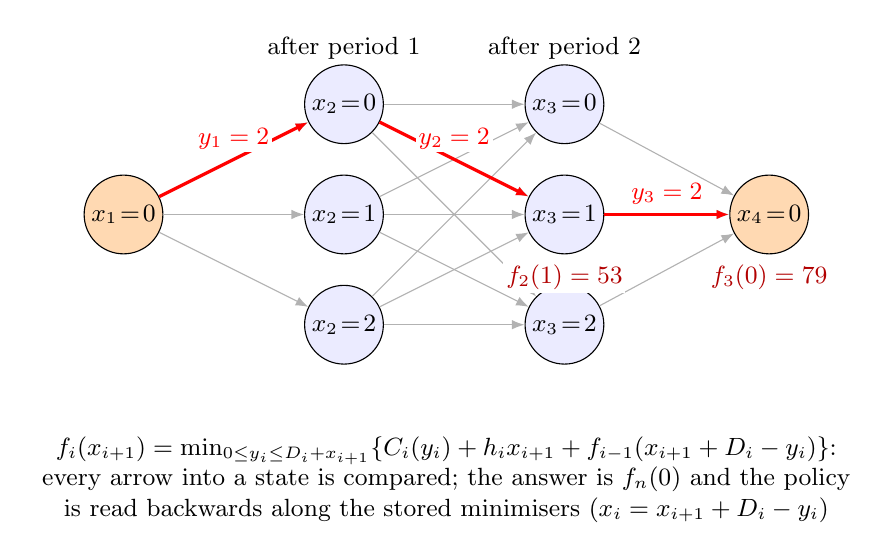
\begin{tikzpicture}[every node/.style={font=\small}, >={Latex[length=1.6mm]}, st/.style={draw, circle, minimum size=10mm, inner sep=0.5pt, font=\small, fill=blue!8}]
	\node[st, fill=orange!30] (s0) at (0,0) {$x_1\!=\!0$};
	\foreach \x in {0,1,2} {\node[st] (a\x) at (2.8,{-1.4*\x+1.4}) {$x_2\!=\!\x$};}
	\foreach \x in {0,1,2} {\node[st] (b\x) at (5.6,{-1.4*\x+1.4}) {$x_3\!=\!\x$};}
	\node[st, fill=orange!30] (c0) at (8.2,0) {$x_4\!=\!0$};
	\foreach \x in {0,1,2} {\draw[->, gray!60] (s0) -- (a\x);}
	\foreach \x in {0,1,2} {\foreach \y in {0,1,2} {\draw[->, gray!60] (a\x) -- (b\y);}}
	\foreach \x in {0,1,2} {\draw[->, gray!60] (b\x) -- (c0);}
	\draw[->, red, very thick] (s0) -- (a0) node[midway, above, font=\small, fill=white, inner sep=1pt, yshift=2pt] {$y_1=2$};
	\draw[->, red, very thick] (a0) -- (b1) node[midway, above, font=\small, fill=white, inner sep=1pt, yshift=2pt] {$y_2=2$};
	\draw[->, red, very thick] (b1) -- (c0) node[midway, above, font=\small, fill=white, inner sep=1pt, yshift=2pt] {$y_3=2$};
	\node[red!70!black, font=\small, anchor=north, fill=white, inner sep=1pt] at (5.6,-0.6) {$f_2(1)=53$};
	\node[red!70!black, font=\small, anchor=north, fill=white, inner sep=1pt] at (8.2,-0.6) {$f_3(0)=79$};
	\node[font=\small, anchor=south] at (2.8,1.85) {after period 1};
	\node[font=\small, anchor=south] at (5.6,1.85) {after period 2};
	\node[anchor=north, align=flush center, text width=10.4cm] at (4.1,-2.7) {$f_i(x_{i+1})=\min_{0\le y_i\le D_i+x_{i+1}}\{C_i(y_i)+h_ix_{i+1}+f_{i-1}(x_{i+1}+D_i-y_i)\}$: every arrow into a state is compared; the answer is $f_n(0)$ and the policy is read backwards along the stored minimisers ($x_i=x_{i+1}+D_i-y_i$)};
\end{tikzpicture}
\end{document}
